
\chapter{Population Study of \Acsptitle{LAT}-detected \Acsptitle{PWN}}

\paperref{This chapter is based the second part of the the paper
  ``Constraints on the Galactic Population of TeV Pulsar Wind Nebulae using Fermi Large Area Telescope Observations''
  by Acero et al which is currently in prep.}

In \chapref{extended_search}, we search for new spatially-extended \fermi
sources and found that spatial extenion was an important characteristic
for detecting new \acp{PWN}. In the process, we discovered three
new $\gamma$-ray emitting \acp{PWN}.  In \chapref{offpeak}, we then
searched in the off-peak phase interval of \ac{LAT}-detected pulsars
for new pulsar wind nebula and discovered \threecfiftyeight.  Finally,
in \chapref{tevcat} we searched in the regions surrounding \acp{PWN}
candidates detected at \tev energies for \gev-emitting \acp{PWN}
4 new PWNe candidates (\hess{J1119}, \hess{J1303}, \hess{J1420},
and \hess{J1841}) and 1 new PWN (\hess{J1356})

In this chapter, we take the population of $\gamma$-ray emitting \acp{PWN} and \acp{PWN}
candidates


\section{Summary of the \Acsptitle{PWN} detected by the \Acsptitle{LAT}}

\section{The Evolution of $\gamma$-ray Emitting \Acsptitle{PWN} with the Properties of their Pulsars}


\begin{figure}[htbp]
  \centering
  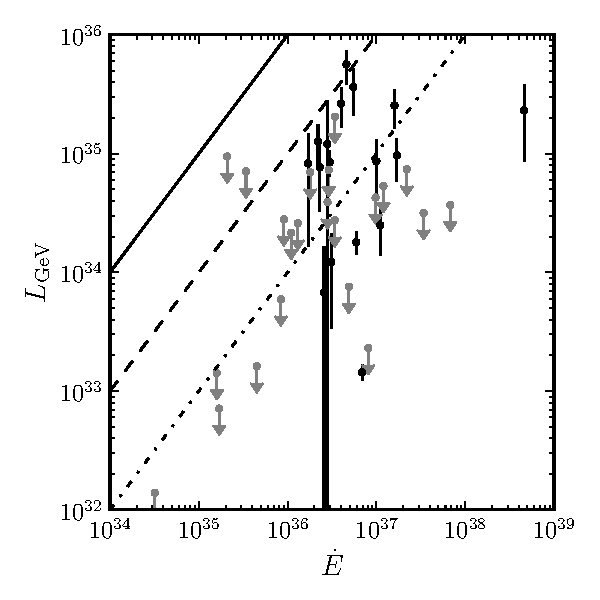
\includegraphics{chapters/population_study/figures/pwn_luminosity_vs_edot.pdf}
  \caption{...}
  \figlabel{pwn_luminosity_vs_edot}
\end{figure}


\begin{figure}[htbp]
  \centering
  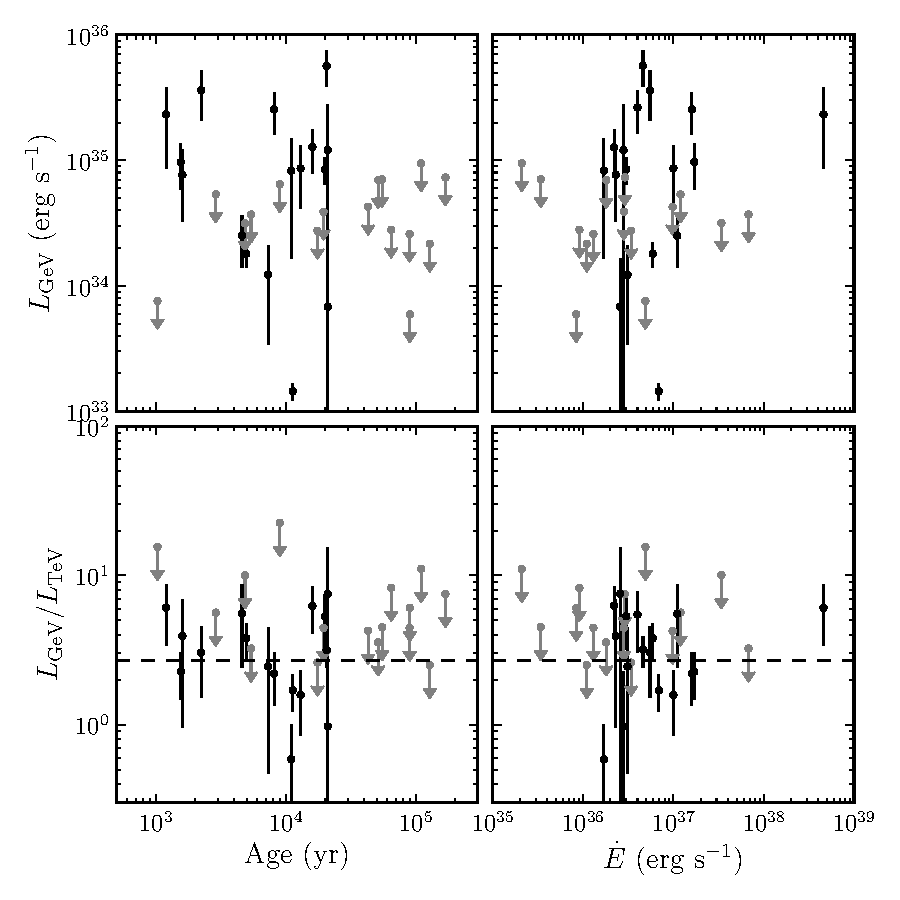
\includegraphics{chapters/population_study/figures/pwn_age_edot_vs_l_gev.pdf}
  \caption{...}
  \figlabel{pwn_age_edot_vs_l_gev.pdf}
\end{figure}


\begin{figure}[htbp]
  \centering
  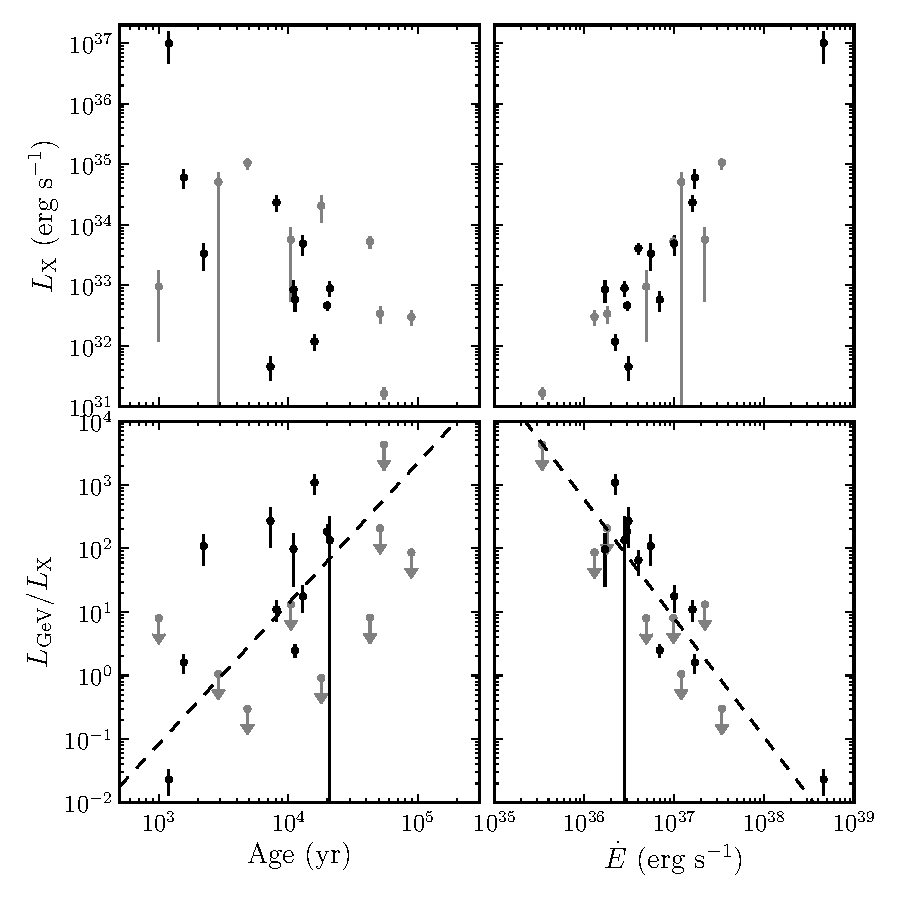
\includegraphics{chapters/population_study/figures/pwn_age_edot_vs_l_xray.pdf}
  \caption{...}
  \figlabel{pwn_age_edot_vs_l_xray}
\end{figure}
